
\subsection{Superconductors and Available Materials}

At the beginning of the \nth{20} century, Heike Kamerlingh Onnes liquified helium and started using it to cool down various metals to extremely low temperatures. He discovered that the resistance of solid mercury disappeared at $T=4.2~\text{K}$ and named this phenomenon a "superconductivity". Since that period, there have been many discovered materials characterised by similar physical properties. There are two main types of superconductors distinguished by the temperature at which they loose their superconducting state: 
\begin{itemize}
    \item Low-temperature superconductors (LTS).
    \item High-temperature superconductors (HTS).
\end{itemize}
LTS-based cables can operate in a superconducting state in the range of $T \in (4, 20)~\text{K}$ whereas HTS-based ones -- at higher temperatures. The HTS technology is very promising for future applications because it will enable machines for an operation at higher magnetic fields while spending less energy to cool it. However, the HTS cables still remain at the stage of research and development in most of the applications concerning accelerator magnets~\cite[p.~77-95]{evans_marvel_of_technology}. 

In order to use a superconductor in engineering applications for a magnet design, it must meet four basic requirements~\cite[p.~77-95]{evans_marvel_of_technology}:

\begin{enumerate}
    \item The material should have appropriate basic physical properties, i.e. high critical temperature and critical magnetic field.
    \item The material must be relatively common, i.e. reasonably cheap.
    \item The material must be easy to form into common shapes such as tapes or wires.
    \item The material must withstand mechanical loads inside a magnet.
\end{enumerate}

There are two low-temperature superconductors that are commercially available for~a large scale magnet production: Nb-Ti and $\text{Nb}_3 \text{Sn}$. Each of them meets most of the specified technical requirements. Nb-Ti is an alloy widely used in a magnet design due to its extreme ductility that allows for an easy cable extrusion and further winding process. $\text{Nb}_3 \text{Sn}$ is a brittle material sensitive to mechanical stresses. It requires a greater effort in coil production compared to Nb-Ti. In the fabrication process, it is initially formed to resemble its final geometry. The next manufacturing step consists of a few day high-temperature treatment during which the cable hardens and reaches its full performance. The main advantage of $\text{Nb}_3 \text{Sn}$ is its higher critical parameters of temperature and magnetic field with respect to Nb-Ti~\cite[p.~29-41]{superconducting_accelerator_magnets}.

\subsection{Critical Parameters and Stability}

As presented in Fig.~\ref{fig:scheme_critical_surface}, the superconducting state depends on three critical parameters: temperature, magnetic field and current density. These three variables create a so called "critical surface" under which a material remains in a superconducting state. The transition from the superconducting to the normal state is called a "quench". It occurs when an operating point of a superconductor remains outside of the critical surface. One can notice in Fig.~\ref{fig:scheme_critical_surface} that $\text{Nb}_3 \text{Sn}$ is characterised by a larger volume under the critical surface. Higher critical parameters of this material allow for its potential usage at stronger fields in accelerator magnets.

\begin{figure}[H]
    \centering
    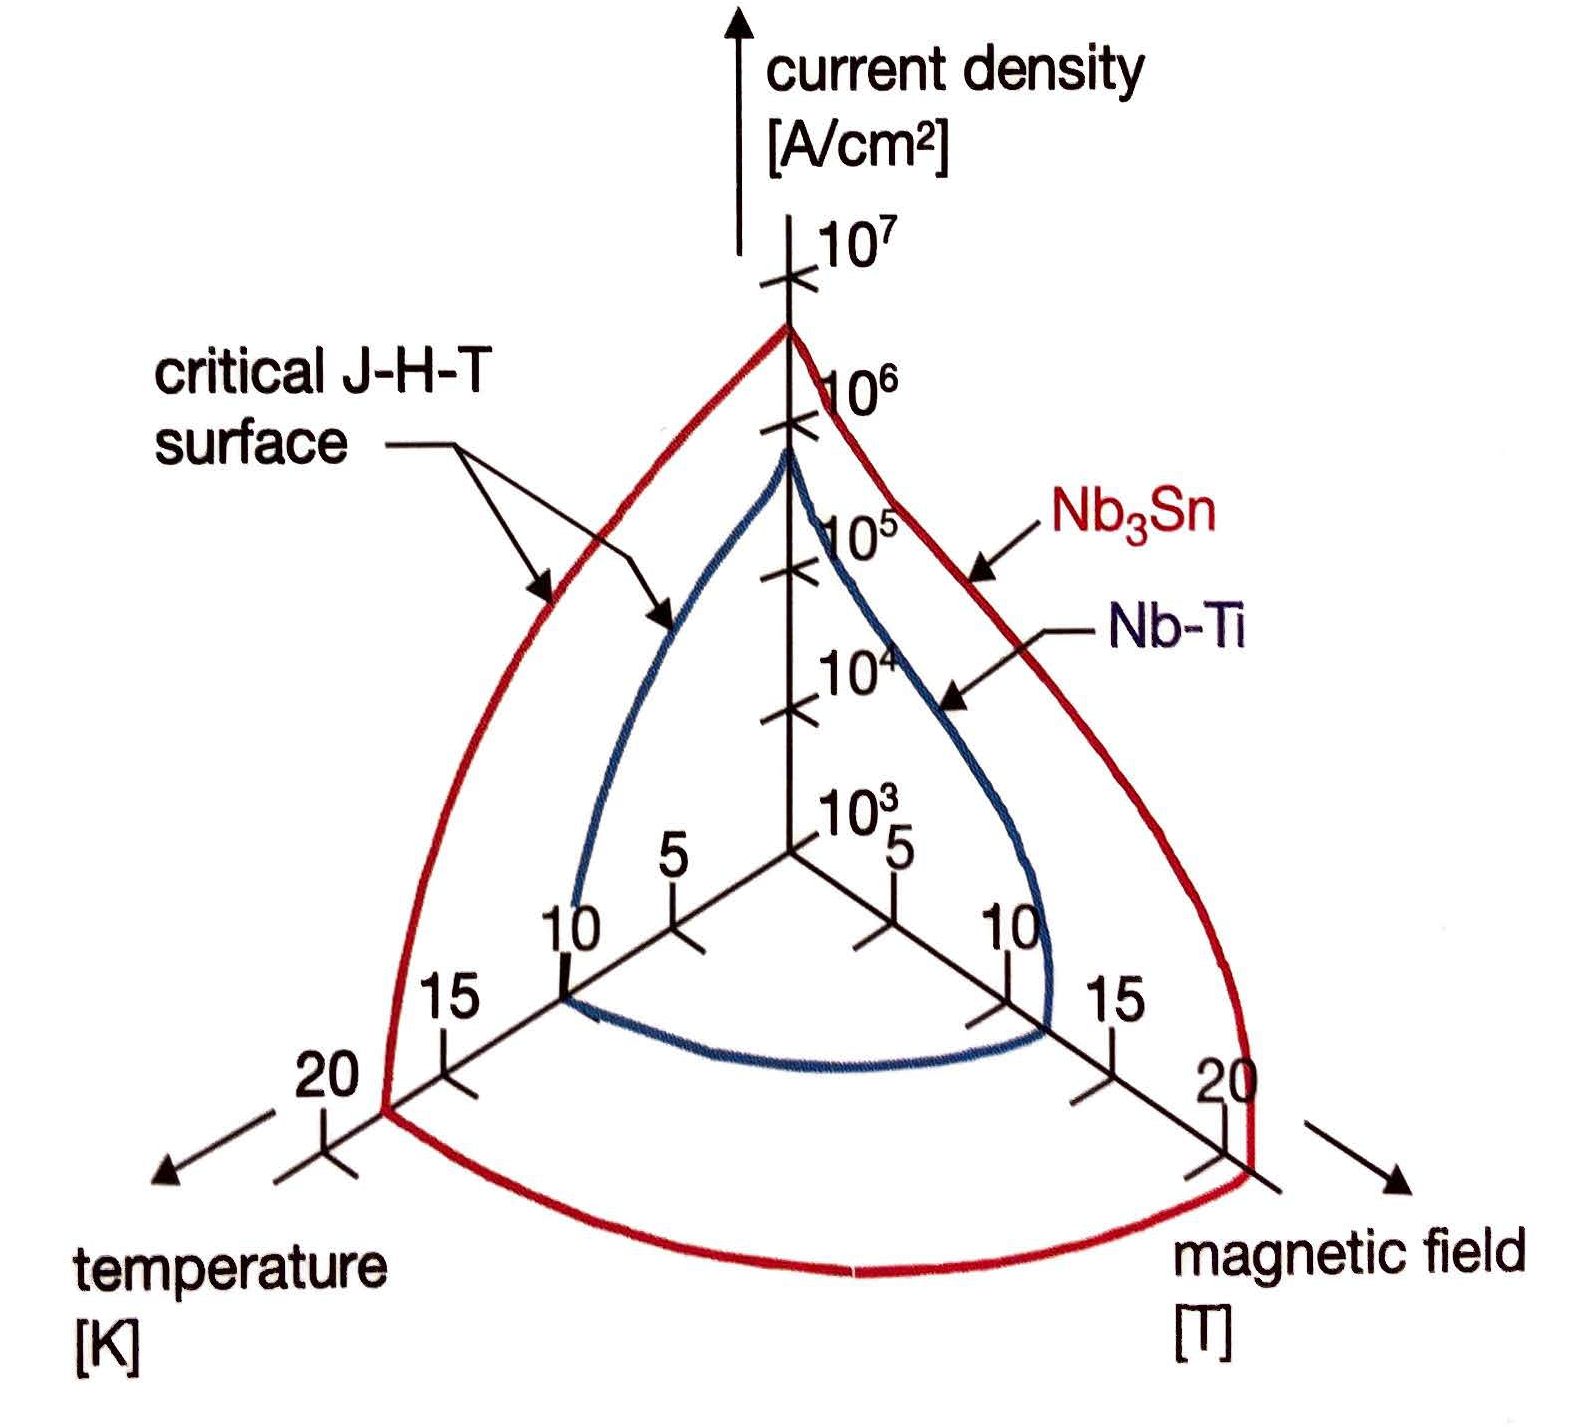
\includegraphics[width=0.35\linewidth]{sections/introduction/figures/critical_surface_scheme.png}
    \caption{Critical surface for $\text{Nb}_\text{3}\text{Sn}$ and Nb-Ti \cite{evans_marvel_of_technology}}
    \label{fig:scheme_critical_surface}
\end{figure} 

From the magnet design standpoint, it is impossible to use a superconductor alone because it is vulnerable to flux jumps. If the material exceeds its critical magnetic field, it looses its superconducting properties. A superconductor can easily reach its critical temperature as well. At temperatures close to the absolute zero, even a small energy deposition in the order of $1~\frac{\text{mJ}}{g}$ may cause a quench. It is mainly due to an extreme low heat capacity of solid materials at cryogenic temperatures (see Appendix~\ref{appendix_material_properties_description}). In addition, superconductors have relatively high resistivity in a normal conducting state with respect to the materials considered to be good electrical conductors such as copper. As described in Fig.~\ref{fig:resitivity_tin_copper}, the resistivity of tin, being a superconductor below $T_\text{c}$, is higher at normal conductive state with respect to the copper~\cite[p.~1-6]{superconducting_accelerator_magnets}.

\begin{figure}[H]
    \centering
    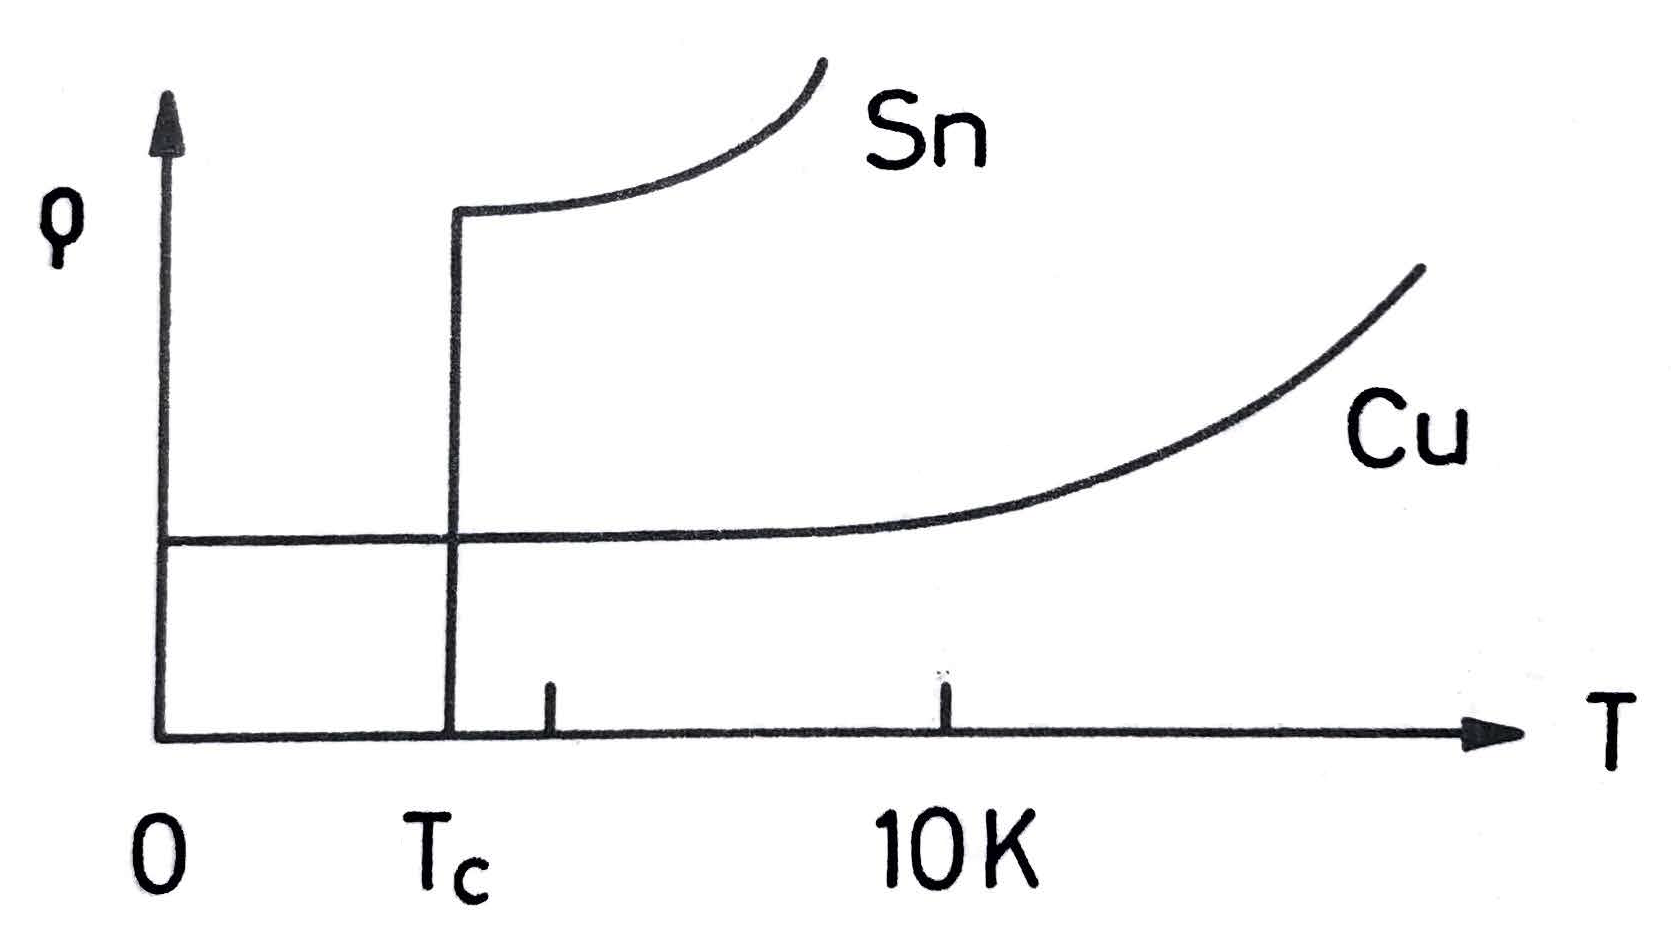
\includegraphics[width=0.35\linewidth]{sections/introduction/figures/sn_cu_resistivity.png}
    \caption{Low temperature resistivity of copper and tin~\cite{superconducting_accelerator_magnets}}
    \label{fig:resitivity_tin_copper}
\end{figure} 

In order to increase the cable stability, a superconductor is embedded in a copper matrix. When a superconductor quenches, the current bypasses it and flows through the copper characterised by a lower resistivity in a normal conducting state. During that moment, the superconductor may cool down and recover its superconducting state. The copper matrix serves for three purposes~\cite[p.~31-33]{superconducting_accelerator_magnets}: 

\begin{enumerate}
    \item Mechanical stability.
    \item Electrical bypass of high electrical conductivity.
    \item Heat sink.
\end{enumerate}

The strand composite of Nb-Ti with a copper matrix is illustrated in two pictures in Fig.~\ref{fig:strand_and_filaments}. In the left one, singular superconductor filaments are shown whereas the right one represents a cross-section of a full strand with Nb-Ti and a copper matrix. The strand diameter is usually approximately equal to 1~mm, and the diameter of a single filament -- $10~\upmu$m.
The composite fabrication should ensure a good contact between the copper and a~superconductor. The copper should also be characterised by a high residual resistivity ratio (see Appendix~\ref{appendix:subsection_rrr_definition}), i.e. it ought to be highly conductive both electrically and thermally~\cite[p.~31-33]{superconducting_accelerator_magnets}.

\begin{figure}[H]
    \centering
    \begin{tikzpicture}
    \node at (5,0) {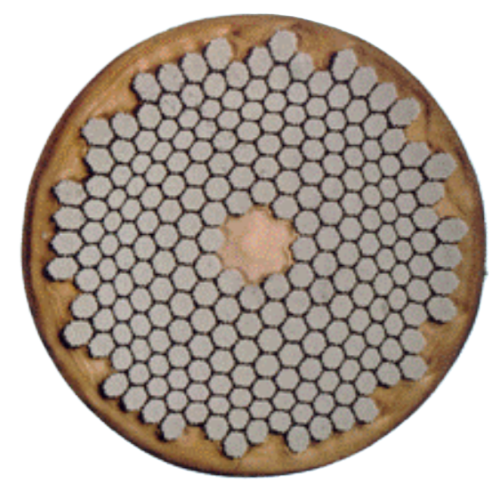
\includegraphics[width=.3\textwidth]{sections/introduction/figures/strand_cross_section.png}};
    \node at (0,0) {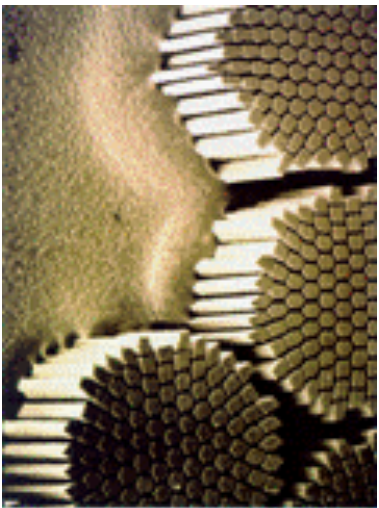
\includegraphics[width=.22\textwidth]{sections/introduction/figures/strand_filaments.png}};
    \end{tikzpicture}
    \caption{Left: Nb-Ti strand cross-section, right: filaments in the strand~\cite{lhc_machine_outreach}}
    \label{fig:strand_and_filaments}
\end{figure}

Another method to increase the strand stability is based on using a cooling liquid. Liquid helium is characterised by a high heat capacity with respect to solids at temperatures close to absolute zero. By assuring a good thermal contact between the strand and the liquid, one can strongly increase the system stability. However, in many applications the strand or a stack of strands is fully insulated with a polymer that does not enable helium to penetrate the copper matrix. In such a case, the direct contact between the liquid and the strand is negligible and cooling of a quenched zone is only possible through a longitudinal heat propagation along the strand~\cite[p.~122]{superconducting_accelerator_magnets}.

Taking into consideration a superconducting magnet as a whole composed of multiple strands, it may quench mainly because of two reasons: 
\begin{enumerate}
    \item A coil element can move in a stack of strands due to the action of Lorentz forces. The friction movement between different elements of the winding  would result in the generation of heat.
    \item According to the Faraday's Law, any change of a magnetic flux in a system creates an electromotive force, (EMF). The EMF induces eddy currents resulting in a magnetic field opposing the initial change of the magnetic flux. Since the composite strands are partially made of copper, being normal conducting at every moment of the magnet operation, excessive eddy currents can be an important heat source for a superconductor.
\end{enumerate}

\subsection{Current Sharing Phenomenon}

In reality, when an operating point of a superconductor starts approaching the critical surface, it exhibits a gradual transition to a normal conducting resistivity. This phenomenon is called current sharing. If the current in the composite strand slightly exceeds the value of a critical current, both elements of the strand become normal conducting. It is assumed that the superconductor carries the current of its critical value and the copper matrix bypasses the surplus of this value equal to $I-I_\text{c}$. In this case, the superconductor and the copper are in a parallel connection~\cite[p.~119-121]{superconducting_accelerator_magnets}. By assuming a linear dependence of $I_\text{c}$ on temperature, the critical current can be calculated as 
\begin{equation}
    I_\text{c} = I \cdot \frac{T-T_\text{cs}}{T_\text{c}-T_\text{cs}},
\end{equation}
where $I_\text{c}$ -- critical current, $I$ -- transport current in the strand, $T$ -- local temperature of the strand, $T_\text{c}$ -- critical temperature, $T_\text{cs}$ -- current sharing temperature. If the local temperature $T$ is assumed to be equal to the operating bath temperature $T_0$, one can deduce the current sharing temperature as
\begin{equation}
    T_\text{cs} = T_\text{0} + (T_\text{c} - T_\text{0}) \cdot (1 - \frac{I}{I_\text{c}~T_0}),
\end{equation}
where $T_0$ -- bath temperature of the strand. Therefore, the current in a copper matrix can be divided into three regimes as
\begin{equation}
    \left\{ \begin{array}{ lll }
    I_\text{Cu} = 0 & \text{for}~T < T_\text{cs}, \\ \\
    I_\text{Cu} = I - I_\text{c} & \text{for}~T_\text{cs} \leq T<T_\text{c},  \\ \\
    I_\text{Cu} = I & \text{for}~T_\text{cs} \leq T,
    \end{array} \right.
\end{equation}
where $I_\text{Cu}$ -- current in the copper matrix. Following the regimes for the current in the copper matrix, one can deduce three regimes for the Joule heating as
\begin{equation}
    \left\{ \begin{array}{lll}
    q_\text{Joule} = 0 & \text{for}~T < T_\text{cs}, \\ \\
    q_\text{Joule} = \frac{\rho_\text{Cu}}{f_\text{Cu}} \cdot \frac{(I-I_\text{c})^2}{{A_\text{Cu}}^2}& \text{for}~T_\text{cs} \leq T<T_\text{c},  \\ \\
    q_\text{Joule} = \frac{\rho_\text{Cu}}{f_\text{Cu}} \cdot \frac{I^2}{{A_\text{Cu}}^2} & \text{for}~T_\text{cs} \leq T,
    \end{array} \right.
\end{equation}
where $q_\text{Joule}$ -- Joule heating, $\rho_\text{Cu}$ -- local resistivity of copper, $f_\text{Cu}$ -- fraction of copper in the composite strand, $A_\text{Cu}$ -- cross-sectional area of copper in the composite strand.

\subsection{Minimum Propagating Zone}

In this section, a fully insulated strand is analysed, i.e. the influence of helium in quench propagation is negligible. In the given consideration, the following assumptions are made: 
\begin{itemize}
    \item The strand is only made of a superconductor without a copper stabiliser. 
    \item The current density in the wire is close to its critical value. 
    \item The length $L$ of a superconductor is heated from the bath temperature $T_0$ to the temperature $T$ above the critical value $T_\text{c}$.
\end{itemize}

Since helium is not considered, the thermal disturbance in the strand leads to the quench propagation if the longitudinal heat evacuation is lower than the generation of heat in the quenched zone. It is formulated as
\begin{equation}
    \rho J^2 A L \geq \frac{kA(T_\text{c}-T_0)}{L},
\end{equation}
where $J$ -- current density, $A$ -- wire cross-section, $L$ -- heated length of a superconductor, $k$~-- thermal conductivity of the wire, $T_\text{c}$ -- critical temperature, $T_0$ -- bath temperature. One can simply deduce the minimum propagating zone from the equation as
\begin{equation}
    L_\text{MPZ} = \sqrt{\frac{2k(T_\text{c}-T_0)}{\rho J^2}}.
\end{equation}
If the thermal disturbance is larger or equal to $L_\text{MPZ}$, the quench starts propagating along the wire. For pure Nb-Ti, the $L_\text{MPZ}$ is approximately equal to $L=1~\upmu \text{m}$. Such a~small value explains why a~copper stabiliser is necessary in a composite strand. The usage of copper may increase $L_\text{MPZ}$ by a factor of thousand~\cite[p.~124]{superconducting_accelerator_magnets}. 